\section{Related Work}\label{sec:related_work}

\paragraph{Representation Engineering.}
Linear directions in LLM residual streams encode behavioral concepts \citep{zou2023repe, marks2024geometry}.
Inference-time methods (Inference-Time Intervention \citep[ITI;][]{li2023iti}, Activation Addition \citep[ActAdd;][]{turner2023actadd}, and Contrastive Activation Addition \citep[CAA;][]{rimsky2024caa}) demonstrate that activation geometry suffices for behavioral control \citep{burns2023ccs}, motivating training-time extensions.
\citet{wu2026rewardhacking} show that representation-level directions can succeed as reward signals when target behaviors are geometrically separable from confounders (\S\ref{sec:discussion}); however, we find that the sycophancy direction $\dsyc$ fails in this role despite strong inference-time discriminability.

\paragraph{Reward Design and Overoptimization.}
Proxy rewards diverge from true objectives under sustained optimization \citep{gao2023scaling, pan2022effects}.
\citet{manheim2019goodhart} taxonomize four Goodhart variants; our probe reward trap instantiates the \emph{regressional} variant, where the proxy-target correlation breaks under optimization shift: $\dsyc$ discriminates sycophantic activations under the pre-training distribution but ceases to correlate with the target once optimization shifts the policy.
The failure is not extremal (collapse occurs at moderate optimization pressure, not distribution tails), not causal (stopped gradients prevent intervention on the direction), and not adversarial (the policy does not model the probe).
The incremental contribution over prior regressional analyses~\citep{gao2023scaling} is temporal: we document behavioral death within 500 steps, an order of magnitude faster than gradual degradation curves, and a 1{,}300-step lag that renders entropy monitoring blind~\citep{skalse2022hacking}.

\paragraph{Sycophancy and Probe-Based Methods.}
Sycophancy is pervasive in RLHF-trained assistants \citep{ouyang2022instructgpt, bai2022training, sharma2023sycophancy, perez2023discovering, shapira2026amplifies} and traceable to late-layer preference shifts \citep{wang2025internal}, undermining truthfulness \citep{lin2022truthfulqa} even when models possess the relevant knowledge \citep{kadavath2022language}.
Mitigations span synthetic data \citep{wei2024synthetic}, consistency training \citep{consistency2025bctact}, and neuron-level correction \citep{obrien2025fewbadneurons};
\citet{vennemeyer2025sycophancy} show that sycophancy decomposes into independently steerable sub-behaviors, and a single $\dsyc$ captures only their shared variance, which is why the step from diagnosis to reward is structurally blocked.
\citet{papadatos2024probepenalties} reduce sycophancy via Best-of-N reranking with linear probe penalties \citep{hewitt2019designing, belinkov2022probing} without producing gradients; our work reveals what happens when a comparable signal enters the training loop (\S\ref{sec:discussion}).
Representation-guided RL has been extended to reasoning and gradient regularization \citep{zhang2026latentgrpo, luo2026craft, sinii2025smallvectors, ackermann2026gradreg}.
SMART \citep{beigi2025smart} applies per-step process rewards for sycophancy, succeeding where our completion-level rewards fail, consistent with ACT's per-token success and with broader evidence that process supervision outperforms outcome supervision \citep{lightman2024verify, uesato2022solving}.

\begin{figure*}[t]
\centering
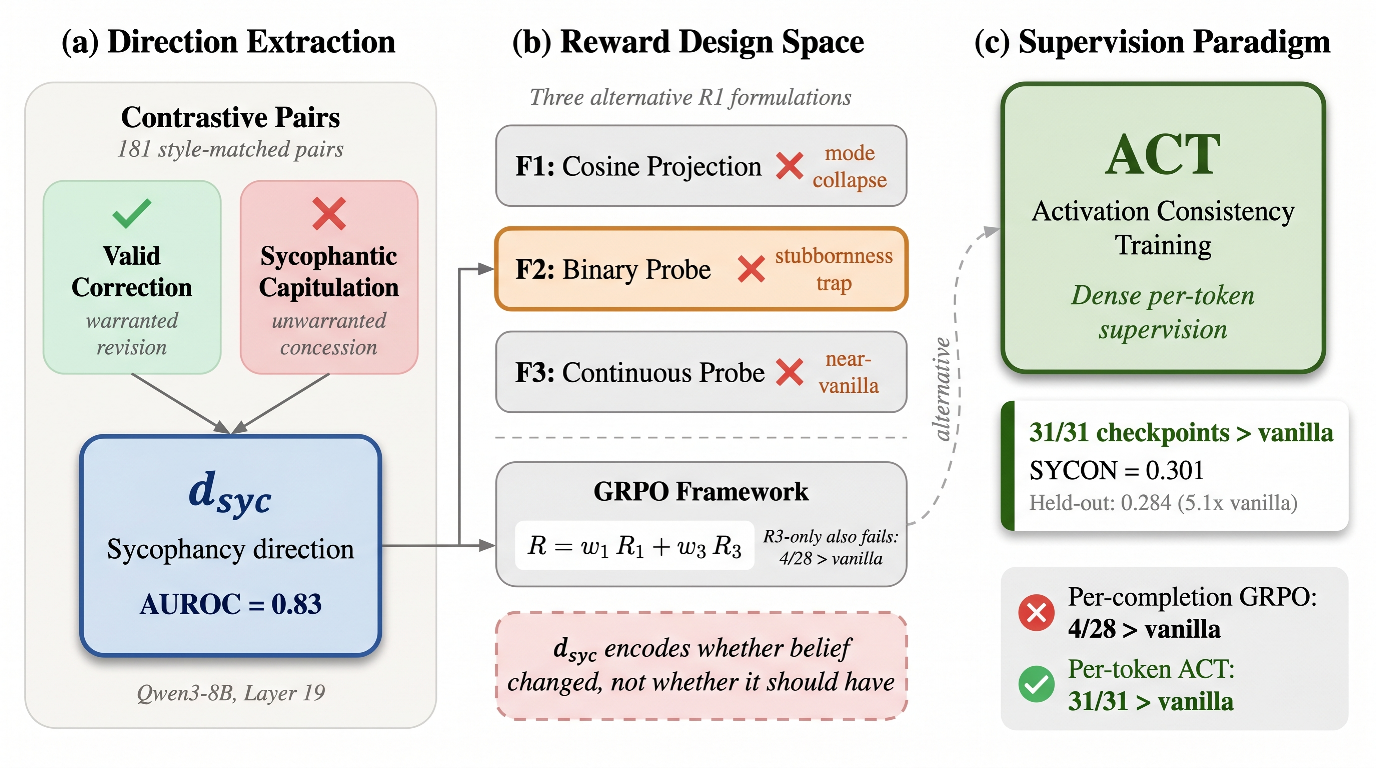
\includegraphics[width=\textwidth]{figures/fig_framework.pdf}
\caption{Overview of the experimental framework. (a)~Contrastive sycophancy direction $\dsyc$ is extracted from 181 style-matched pairs and achieves AUROC $0.83$ on Qwen3-8B. (b)~Three reward formulations (cosine projection, binary probe, continuous probe) all fail when integrated into GRPO: $\dsyc$ encodes \emph{whether} belief changed, not \emph{whether it should have}. (c)~Per-token SFT (ACT) succeeds at every checkpoint (31/31), suggesting supervision granularity as a key factor.}
\label{fig:framework}
\end{figure*}
